\documentclass[12pt]{article}
% Comment the following line to NOT allow the usage of umlauts
\usepackage{bm}
\usepackage{hyperref}
\usepackage{amssymb}
\usepackage{amsthm}
\usepackage{amsmath} \let\oldforall\forall \let\forall\undefined \DeclareMathOperator{\forall}{\oldforall}
\renewcommand{\vec}[1]{\bm{\mathrm{#1}}}
\usepackage[shortlabels]{enumitem}
\usepackage[margin=1in]{geometry}
\usepackage{theoremref}
\usepackage{setspace}
\onehalfspacing
\setlength{\jot}{10pt}

%encoding
%--------------------------------------
\usepackage[utf8]{inputenc}
%--------------------------------------
\usepackage{xcolor}
\usepackage{listings}

\definecolor{mGreen}{rgb}{0, 0.6, 0}
\definecolor{mGray}{rgb}{0.5, 0.5, 0.5}
\definecolor{mPurple}{rgb}{0.58, 0, 0.82}
\definecolor{backgroundColour}{rgb}{0.95, 0.95, 0.92}

\lstdefinestyle{Python}{
    backgroundcolor=\color{backgroundColour},   
    commentstyle=\color{mGreen},
    keywordstyle=\color{magenta},
    numberstyle=\tiny\color{mGray},
    stringstyle=\color{mPurple},
    basicstyle=\footnotesize,
    breakatwhitespace=false,         
    breaklines=true,                 
    captionpos=b,                    
    keepspaces=true,                 
    numbers=left,                    
    numbersep=5pt,                  
    showspaces=false,                
    showstringspaces=false,
    showtabs=false,                  
    tabsize=2,
    basicstyle=\ttfamily\footnotesize,
    language=Python
}
%--------------------------------------
\usepackage{graphicx}
\title{Faster approach to evaluate nested sums of polynomials}
\author{Pedro Cleto \\ \href{mailto:cl3t0.sh@gmail.com}{cl3t0.sh@gmail.com} }
\date{March 2024}

% Start the document
\begin{document}

\newtheorem{theorem}{Theorem}
\newtheorem{corollary}{Corollary}[theorem]
\newtheorem{lemma}[theorem]{Lemma}

\maketitle

\section{Abstract}

In this paper, we show 4 algorithms to evaluate nested sums of polynomials. The last two are the main work of this paper. Define $f$ and $S$ as

\begin{align*}
    f(x)       & := a_0 + a_1 x + a_2 x^2 + \cdots + a_n x^n                               \\
    S(a, b, k) & := \sum_{i_1=a}^{b}\sum_{i_2=a}^{i_1}\cdots\sum_{i_k=a}^{i_{k-1}} f(i_k).
\end{align*}

The first algorithm consists of evaluating in a naive way, applying summations using recursion. Let's call it "Naive sum". The second one uses memoization and is what probably most people thought to use because it's not hard to think and it hugely optimizes running time and depends almost equally on $b - a$, $k$, and $n$. Let's call it "Memoized sum". The third algorithm transforms the summations into a single summation using binomial coefficients so the running time does not depend on $k$. Let's call it "BCS" (Binomial Coefficients Sum). Finally, the fourth algorithm exploits the fact that $f$ is polynomial and uses binomial coefficients and matrices operations to depend mostly on $n$. It means that this algorithm is faster for bigger $k$ and $b - a$ and small $n$. Let's call it "BCBTS" (Binomial Coefficients Base Transformation Sum).

\section{Algorithm 1: Naive Sum}

\subsection{Code and complexity analysis}

The algorithm is brute force so it doesn't require proof. Python is not the fastest programming language but we are using it only for comparison purposes and to avoid float precision problems.

\begin{lstlisting}[style=Python]
from typing import List


def nested_sum_of_polynomial(
    a: int,
    b: int,
    k: int,
    f_coefs: List[float],
) -> float:
    def func(x: int) -> int:
        # Horner's method for polynomial evaluation
        acc = f_coefs[-1]
        for coef in f_coefs[-2::-1]:
            acc *= x
            acc += coef
        return acc

    def recursive_sum(x: int, k: int) -> float:
        res = (
            func(x) if k == 0 else sum(recursive_sum(i, k - 1) for i in range(a, x + 1))
        )
        return res

    return recursive_sum(b, k)


result = nested_sum_of_polynomial(
    a=1,
    b=100,
    k=4,
    f_coefs=[5, -1, 1, -5, -3, 3],  # Put your function coefficients here
)

print(result)

\end{lstlisting}

Note that it's a simple and short code but extremely inefficient due to function recursion. Doing some analysis we conclude that the time complexity of this algorithm is $O\Big(n \binom{b-a+k-1}{k}\Big)$ given $a, b, k, n$. It's not precise because Python doesn't do exactly what we order. Because of this, we are going to do some practical comparisons at the end.

\section{Algorithm 2: Memoized Sum}

\subsection{Code and complexity analysis}

Here we are going to rewrite the same algorithm as before but with memoization.

\begin{lstlisting}[style=Python]
from typing import List


def nested_sum_of_polynomial(
    a: int,
    b: int,
    k: int,
    f_coefs: List[float],
) -> float:
    mem = {}

    def func(x: int) -> int:
        # Horner's method for polynomial evaluation
        acc = f_coefs[-1]
        for coef in f_coefs[-2::-1]:
            acc *= x
            acc += coef
        return acc

    def recursive_sum(x: int, k: int) -> float:
        if mem.get((x, k)) is not None:
            return mem[(x, k)]

        res = (
            func(x) if k == 0 else sum(recursive_sum(i, k - 1) for i in range(a, x + 1))
        )
        mem[(x, k)] = res
        return res

    return recursive_sum(b, k)


result = nested_sum_of_polynomial(
    a=1,
    b=100,
    k=4,
    f_coefs=[5, -1, 1, -5, -3, 3],  # Put your function coefficients here
)

print(int(result))
    
\end{lstlisting}

This simple technique drastically speeds things up. Doing some analysis we conclude that the time complexity of this algorithm is $O\Big((b - a)(n + k)\Big)$ given $a, b, k, n$. Again, it's not precise.

\section{Algorithm 3: BCS (Binomial Coefficients Sum)}

\subsection{Presentation}

BCS consists of representing nested sums as binomial coefficients. Its calculation is super simple.

$$
    S(a, b, k) = \sum_{i=a}^{b} f(i) \binom{b + k - 1 - i}{k - 1}
$$

\subsection{Code and complexity analysis}

Note that we can calculate binomial coefficients based on the last coefficient used to reuse computation.

\begin{lstlisting}[style=Python]
from typing import List


def nested_sum_of_polynomial(
    a: int,
    b: int,
    k: int,
    f_coefs: List[float],
) -> float:

    def func(x: int) -> int:
        # Horner's method for polynomial evaluation
        acc = f_coefs[-1]
        for coef in f_coefs[-2::-1]:
            acc *= x
            acc += coef
        return acc

    pascal = 1  # (k - 1 choose k - 1)
    res = 0
    for i in range(a, b + 1):
        res += pascal * func(a + b - i)
        pascal *= (k + i - a) / (i - a + 1)
    return res


result = nested_sum_of_polynomial(
    a=1,
    b=100,
    k=4,
    f_coefs=[5, -1, 1, -5, -3, 3],  # Put your function coefficients here
)

print(int(result)) 
\end{lstlisting}

The code is simple and extremely efficient. After analysis, we know that the time complexity of this algorithm is $O\Big(n (b - a)\Big)$ given $a, b, k, n$. You are not seeing it wrong. This algorithm does \textbf{not} depend on $k$ and is linear on $n$ and $b-a$. BCS is fast enough for most cases, but we are not going to stop here. Before presenting the next algorithm, let's prove BCS works.

\subsection{Proof}

First, we need some auxiliary results.

\begin{theorem}[Pascal's rule]
    \label{pascal_rule}

    For all $i, j \in \mathbb{N}$ where $j < i$ it holds that

    $$
        \binom{i}{j} + \binom{i}{j+1} = \binom{i+1}{j+1}.
    $$

\end{theorem}

\begin{proof}

    By developing and manipulating the binomial coefficients, we get

    \begin{align*}
        \binom{i}{j} + \binom{i}{j+1} & = \frac{i!}{j!(i-j)!} + \frac{i!}{(j+1)!(i-(j+1))!}           \\
                                      & = \frac{i!(j+1)}{(j+1)!(i-j)!} + \frac{i!(i-j)}{(j+1)!(i-j)!} \\
                                      & = \frac{i!(i+1)}{(j+1)!(i-j)!}                                \\
                                      & = \frac{(i+1)!}{(j+1)!((i+1)-(j+1))!}.
    \end{align*}

    Therefore,

    $$
        \boxed{\binom{i}{j} + \binom{i}{j+1} = \binom{i+1}{j+1}}.
    $$

\end{proof}

\vspace{20px}

\begin{theorem} [Hockey-stick identity]
    \label{hockey_stick_identity}

    For all $n, a, b \in \mathbb{N}$ where $b \geq a$ it holds that

    $$
        \sum_{i=a}^{b} \binom{i+n-a}{n} = \binom{b+n+1-a}{n+1}.
    $$

\end{theorem}

\begin{proof}

    For $b = a$,


    \begin{align*}
        \sum_{i=a}^{a} \binom{i+n-a}{n} & = \binom{n}{n}          \\
                                        & = 1                     \\
                                        & = \binom{n+1}{n+1}      \\
                                        & = \binom{b+n+1-a}{n+1}.
    \end{align*}

    Therefore,

    $$
        \sum_{i=a}^{a} \binom{i+n-a}{n} = \binom{b+n+1-a}{n+1}.
    $$

    That is, it holds for $b = a$. Suppose it holds for some $b \in \mathbb{N}$ where $b \geq a$. Therefore,


    $$
        \sum_{i=a}^{b} \binom{i+n-a}{n} = \binom{b+n+1-a}{n+1}.
    $$

    Adding $\displaystyle\binom{(b+1)+n-a}{n}$ to both sides we get

    $$
        \sum_{i=a}^{b+1} \binom{i+n-a}{n} = \binom{b+n+1-a}{n+1} + \binom{b+n+1-a}{n}.
    $$

    By the theorem \ref{pascal_rule},

    $$
        \boxed{\sum_{i=a}^{b+1} \binom{i+n-a}{n} = \binom{(b+1)+n-a}{n+1}}.
    $$

    Therefore, it holds for $b + 1$. By the principle of finite induction, it holds for all $b \in \mathbb{N}$ where $b \geq a$.

\end{proof}

Now we are going to show that BCS works for $k = 1$.

\begin{align*}
    S(a, b, 1) & = \sum_{i = a}^{b} f(i) \\
    & = \sum_{i = a}^{b} f(i) \binom{b + 1 - 1 - i}{1 - 1}.
\end{align*}

Suppose that BCS works for some $k \in \mathbb{Z}_{+}$.

\begin{align*}
    S(a, b, k) & = \sum_{i = a}^{b} f(i) \binom{b + k - 1 - i}{k - 1} \\
    \sum_{j=a}^{b} S(a, j, k) & = \sum_{j=a}^{b} \sum_{i = a}^{j} f(i) \binom{j + k - 1 - i}{k - 1} \\
    S(a, b, k + 1) & = \sum_{i=a}^{b} f(i) \sum_{j = i}^{b} \binom{j + k - 1 - i}{k - 1}.
\end{align*}

By the theorem \ref{hockey_stick_identity} we have

$$
    \boxed{S(a, b, k + 1) = \sum_{i=a}^{b} f(i) \binom{b + k - i}{k}}.
$$

Therefore, BCS works for $k + 1$. By the principle of finite induction, BCS works for all $k \in \mathbb{Z}_{+}$.

$\hfill\blacksquare$

\section{Algorithm 4: BCBTS (Binomial Coefficients Base Transformation Sum)}

\subsection{Presentation}

BCBTS consists of rewriting $S$ through binomial coefficients.

$$
    S(a, b, k) = \begin{bmatrix}
        \binom{b+k-a}{k} & \binom{b+1+k-a}{1+k} & \cdots & \binom{b+n+k-a}{n+k}
    \end{bmatrix} \Omega
    \begin{bmatrix}
        a_0 \\ a_1 \\ \vdots \\ a_n
    \end{bmatrix}
$$

where $\Omega$ is an $(n+1) \times (n+1)$ upper triangular matrix defined by the recurrence


\begin{itemize}
    \item $\Omega_{1, 1} := 1$;
    \item For all $i, j \in \mathbb{Z_+}$ where  $j < i \leq n+1$, $\Omega_{i, j} := 0$; \hfill (upper triangular matrix)
    \item For all $i, j \in \mathbb{N}$ where $i, j \leq n$, $\Omega_{i+1, j+1} :=  \Omega_{i, j} i - \Omega_{i+1, j} (i+1-a)$.
\end{itemize}

For example, when $a = 1$ we get

$$
    \Omega =
    \begin{bmatrix}
        1      & 0      & 0      & 0      & 0      & 0      & \cdots \\
        0      & 1      & -1     & 1      & -1     & 1      & \cdots \\
        0      & 0      & 2      & -6     & 14     & -30    & \cdots \\
        0      & 0      & 0      & 6      & -36    & 150    & \cdots \\
        0      & 0      & 0      & 0      & 24     & -240   & \cdots \\
        0      & 0      & 0      & 0      & 0      & 120    & \cdots \\
        \vdots & \vdots & \vdots & \vdots & \vdots & \vdots & \ddots
    \end{bmatrix}.
$$

\vspace{20px}

\subsection{Code and complexity analysis}

\begin{lstlisting}[style=Python]
import numpy as np
from typing import List


def nested_sum_of_polynomial(a: int, b: int, k: int, f_coefs: List[float]) -> float:
    n = len(f_coefs) - 1
    coefs_vec = np.array([0, *f_coefs]).reshape(-1, 1)

    # calculating pascal triangle elements
    last_val = 1  # (b + k - a choose 0)
    for i in range(k):
        last_val *= (b + k - a - i) / (i + 1)

    # calculating base vector values
    base = [0, last_val]
    # (b + k - a choose k)
    for i in range(2, n + 2):
        base.append(base[i - 1] * (b + k + i - 1 - a) / (k + i - 1))
    base_vec = np.array(base).reshape(1, -1)

    # initializing omega matrix
    omega = np.zeros(shape=(n + 2, n + 2))
    omega[1, 1] = 1

    # calculating omega matrix
    for j in range(2, n + 2):
        for i in range(1, j + 1):
            omega[i, j] = (i - 1) * omega[i - 1, j - 1] - (i - a) * omega[i, j - 1]

    result = np.linalg.multi_dot([base_vec, omega, coefs_vec])
    return result[0, 0]


result = nested_sum_of_polynomial(
    a=1,
    b=100,
    k=4,
    f_coefs=[5, -1, 1, -5, -3, 3],  # Put your function coefficients here
)

print(int(result))
    
\end{lstlisting}

This time it is possible to notice a more extensive code and more operations than algorithm 2 for small $k$ and $b$. Doing some analysis we conclude that the time complexity of this algorithm is $O\Big(k + n^2\Big)$ given $a, b, k, n$. It means that it does not depend on $b$ and $a$ and depends linearly on $k$. This algorithm seems ideal for small $n$, big $k$, and arbitrarily large $b - a$.

\subsection{Proof}

To represent summations in an alternative way we need to show some intermediate results.

\vspace{20px}

\begin{theorem}
    \label{expanded_hockey_stick_identity}

    For all $n, a, b \in \mathbb{N}$ where $b \geq a$ and $k \in \mathbb{Z_+}$ it holds that

    $$
        \sum_{i_1=a}^{b}\sum_{i_2=a}^{i_1} \cdots \sum_{i_k=a}^{i_{k-1}} \binom{i_k+n-a}{n} = \binom{b+n+k-a}{n+k}.
    $$

\end{theorem}

\begin{proof}

    The case $k = 1$ is already proven by the theorem \ref{hockey_stick_identity}. Suppose that it holds for some $k \in \mathbb{Z_+}$. Therefore,

    $$
        \sum_{i_1=a}^{b}\sum_{i_2=a}^{i_1} \cdots \sum_{i_k=a}^{i_{k-1}} \binom{i_k+n-a}{n} = \binom{b+n+k-a}{n+k}.
    $$

    By summing the expressions for $b$ from $1$ to $m$ on both sides, we get

    $$
        \sum_{b=1}^{m} \left( \sum_{i_1=a}^{b}\sum_{i_2=a}^{i_1} \cdots \sum_{i_k=a}^{i_{k-1}} \binom{i_k+n-a}{n} \right) = \sum_{b=1}^{m} \binom{b+n+k-a}{n+k}.
    $$

    Again using the theorem \ref{hockey_stick_identity}, we know that

    $$
        \sum_{b=1}^{m} \sum_{i_1=a}^{b}\sum_{i_2=a}^{i_1} \cdots \sum_{i_k=a}^{i_{k-1}} \binom{i_k+n-a}{n} = \binom{m+n+k+1-a}{n+k+1}.
    $$

    Changing the notation, we get

    $$
        \boxed{\sum_{i_1=a}^{b} \sum_{i_2=a}^{i_1}\sum_{i_3=a}^{i_2} \cdots \sum_{i_{k+1}=a}^{i_k} \binom{i_{k+1}+n-a}{n} = \binom{b+n+(k+1)-a}{n+(k+1)}}.
    $$

    So it holds for $k+1$. Therefore, by the principle of finite induction, it holds for all $k \in \mathbb{Z_+}$.

\end{proof}

\vspace{20px}

\begin{lemma}
    \label{binomial_degree}

    Let $n \in \mathbb{N}$. Then there exists a polynomial with rational coefficients $p_n \in \mathbb Q[x]$, such that $p_n$ has degree $n$ and for all $x\in \mathbb{N}$ where $x \geq a$, it holds that $p_n(x) = \binom{x+n-a}{n}$.

\end{lemma}

\begin{proof}

    For $n = 0$, define $p_0(x) := 1$. Note that

    $$
        \binom{x-a}{0} = \frac{(x-a)!}{0!(x-a)!} = 1.
    $$

    Therefore, for all $x \in \mathbb{N}$ where $x \geq a$, $p_0(x) = \binom{x-a}{0}$, so it holds for $n = 0$. Suppose it holds for some $n \in \mathbb{N}$. Note that

    \begin{align*}
        \binom{x+n-a}{n}                                                   & = \frac{(x+n-a)!}{n!(x+n-a-n)!}               \\
        \frac{x+n+1-a}{n+1}\binom{x+n-a}{n}                                & = \frac{(x+n+1-a)!}{(n+1)!(x+n-a-n)!}         \\
        \frac{x+n+1-a}{n+1}\binom{x+n-a}{n}                                & = \frac{(x+n+1-a)!}{(n+1)!((x+n+1-a)-(n+1))!} \\
        \left( \frac{1}{n+1}x + \frac{n+1-a}{n+1} \right) \binom{x+n-a}{n} & = \binom{x+n+1-a}{n+1}.
    \end{align*}

    Define

    $$
        p_{n+1}(x) := \left( \frac{1}{n+1}x + \frac{n+1-a}{n+1} \right)p_n(x).
    $$

    Therefore, for all $\displaystyle x \in \mathbb{N}$ where $x \geq a$, $\displaystyle p_{n+1}(x) = \binom{x+n+1-a}{n+1}$, so it holds for $n+1$. By the principle of finite induction, it holds for all $n \in \mathbb{N}$.

\end{proof}

\vspace{20px}

\begin{lemma}
    \label{degree_elevation_identity}

    For all $i, a, x \in \mathbb{N}$ where $x \geq a$ it holds that

    $$
        (i+1)\binom{x+i+1-a}{i+1} - (i+1-a)\binom{x+i-a}{i} = x\binom{x+i-a}{i}.
    $$

\end{lemma}

\vspace{20px}

\begin{proof}

    By developing and manipulating the binomial coefficients, we get

    \begin{align*}
        (i+1)\binom{x+i+1-a}{i+1} - (i+1-a)\binom{x+i-a}{i} & = (i+1)\frac{(x+i+1-a)!}{(i+1)!(x-a)!} - (i+1-a)\frac{(x+i-a)!}{i!(x-a)!} \\
                                                            & = (x+i+1-a)\frac{(x+i-a)!}{i!(x-a)!} - (i+1-a)\frac{(x+i-a)!}{i!(x-a)!}   \\
                                                            & = x\frac{(x+i-a)!}{i!(x-a)!}.
    \end{align*}

    Therefore,

    $$
        \boxed{(i+1)\binom{x+i+1-a}{i+1} - (i+1-a)\binom{x+i-a}{i} = x\binom{x+i-a}{i}}.
    $$

\end{proof}

\vspace{20px}

\begin{theorem}
    \label{polynomial_li}

    For every $n \in \mathbb{N}$ let $p_0,\ p_1,\ p_2,\ \cdots,\ p_n$ such that $p_i$ has degree $i$ for all $i \in \mathbb{N}$ where $i \leq n$. $\displaystyle P = \{ p_0,\ p_1,\ p_2,\ \cdots,\ p_n \}$ is linearly independent in $P_n(\mathbb{C})$.

\end{theorem}

\begin{proof}

    For $n = 0$,

    $$
        P = \{ p_0 \}.
    $$

    Since the set has only one element, it is linearly independent. Suppose that $P$ is linearly independent for some $n \in \mathbb{N}$. Let $\alpha_0,\ \alpha_1,\ \alpha_2,\ \cdots, \alpha_n,\ \alpha_{n+1} \in \mathbb{C}$ such that

    \begin{align*}
        \alpha_0 p_0 + \alpha_1 p_1 + \cdots  + \alpha_n p_n + \alpha_{n+1} p_{n+1} = 0 \\
        \alpha_0 p_0 + \alpha_1 p_1 + \cdots  + \alpha_n p_n = -\alpha_{n+1} p_{n+1}    \\
    \end{align*}

    The left-hand side has a maximum degree of $n$. Note that if $\alpha_{n+1} \ne 0$ the right-hand side of the equation will have degree $n+1$, which is absurd. Therefore $\alpha_{n+1} = 0$. Applying this new information to the equation, we get

    $$
        \alpha_0 p_0 + \alpha_1 p_1 + \alpha_2 p_2 + \cdots + \alpha_n p_n = 0.
    $$

    By hypothesis, this equation has a unique solution in $\alpha_0 = \alpha_1 = \cdots = \alpha_n = 0$. Thus, it is concluded that $P$ is also linearly independent for $n+1$. By the principle of finite induction, $P$ is linearly independent for all $n \in \mathbb{N}$.

\end{proof}

\vspace{20px}

\begin{corollary}
    \label{simple_polynomial_li}
    For all $n \in \mathbb{N}$, $\displaystyle A = \{ 1,\ x,\ x^2,\ x^3,\ \cdots,\ x^n \}$ is linearly independent in $P_n(\mathbb{C})$.
\end{corollary}

\begin{corollary}
    \label{binomial_li}
    Let $\displaystyle \binom{x+i-a}{i}$ be understood as the polynomial described in lemma \ref{binomial_degree}. For all $n \in \mathbb{N}$, $\displaystyle B = \left\{ \binom{x-a}{0},\ \binom{x+1-a}{1},\ \binom{x+2-a}{2},\ \cdots ,\ \binom{x+n-a}{n} \right\}$ is linearly independent in $P_n(\mathbb{C})$.

\end{corollary}

\begin{proof}
    The proof is given by the theorem \ref{polynomial_li}.
\end{proof}

\vspace{20px}

Given that $n \in \mathbb{N}$ is fixed, we have,
\begin{align*}
    A & = \{ 1,\ x,\ x^2,\ x^3,\ \cdots,\ x^n \}                                                             \\
    B & = \left\{ \binom{x-a}{0},\ \binom{x+1-a}{1},\ \binom{x+2-a}{2},\ \cdots ,\ \binom{x+n-a}{n} \right\}
\end{align*}

These, according to the corollaries \ref{simple_polynomial_li} and \ref{polynomial_li}, are bases of the same vector space $P_n(\mathbb{C})$, therefore there exists a matrix $\Omega$ that performs the base change from $A$ to $B$.

\vspace{20px}

\begin{theorem}

    $\Omega$ is a matrix defined by

    \begin{enumerate}[(a)]
        \item $\Omega_{1, 1} := 1$;
        \item For all $i, j \in \mathbb{Z_+}$ where  $i > j$, $\Omega_{i, j} := 0$; \hfill ($\Omega$ is an upper triangular matrix)
        \item For all $i, j \in \mathbb{N}$, $\Omega_{i+1, j+1} :=  \Omega_{i, j} i - \Omega_{i+1, j} (i+1-a)$.
    \end{enumerate}

\end{theorem}

\begin{proof}

    To make $\Omega$ explicit, it is necessary to analyze how each element of the set $A$ is written in the base $B$, representing each column of $\Omega$. Therefore, it is known by the definition of $\Omega$ that for every $j \in \mathbb{Z_+}$, where $j \leq n+1$, it holds that

    $$
        x^{j-1} = \sum_{i = 0}^{n}\Omega_{i+1,j}\binom{x+i-a}{i}.
    $$

    As $j-1 \leq n$, we can separate the summation into two parts. That is,

    $$
        x^{j-1} = \sum_{i = 0}^{j-1}\Omega_{i+1,j}\binom{x+i-a}{i} + \sum_{i = j}^{n}\Omega_{i+1,j}\binom{x+i-a}{i}.
    $$

    Suppose that for some $i > j$, $\Omega_{i, j} \ne 0$. Note that, because of the assumption, some term of the second summation has degree bigger than $j-1$, which is absurd because the left-hand side of the equation has degree $j-1$. Therefore, for $i > j$, $\Omega_{i, j} = 0$, proving (b). Hence, $x^{j-1}$ can be written as

    \begin{equation}
        x^{j-1} = \sum_{i = 0}^{j-1}\Omega_{i+1,j}\binom{x+i-a}{i}.
    \end{equation}

    Choosing $j = 1$ we have,

    \begin{align*}
        x^0 & = \sum_{i = 0}^{0}\Omega_{i+1,1}\binom{x+i-a}{i} \\
        1   & = \Omega_{1,1}\binom{x-a}{0}                     \\
        1   & = \Omega_{1,1}
    \end{align*}

    proving (a). Multiplying both sides of equation 1 by $x$ we get

    $$
        x^j = \sum_{i = 0}^{j-1}\Omega_{i+1,j}x\binom{x+i-a}{i}.
    $$

    Applying lemma \ref{degree_elevation_identity} we get

    \begin{align*}
        x^j & = \sum_{i = 0}^{j-1}\Omega_{i+1,j} \left( (i+1)\binom{x+i+1-a}{i+1} - (i+1-a)\binom{x+i-a}{i} \right)                    \\
            & = \sum_{i = 0}^{j-1}\Omega_{i+1,j} (i+1)\binom{x+i+1-a}{i+1} - \sum_{i = 0}^{j-1} \Omega_{i+1,j} (i+1-a)\binom{x+i-a}{i} \\
            & = \sum_{i = 1}^{j}\Omega_{i,j} i \binom{x+i-a}{i} - \sum_{i = 0}^{j-1} \Omega_{i+1,j} (i+1-a) \binom{x+i-a}{i}
    \end{align*}

    Since $\Omega_{0,j} 0 \binom{x+0-a}{0} = 0$ and $\Omega_{j+1,j} (j+1-a) \binom{x+j-a}{j} = 0$, it is possible to change the lower limit of the first sum to $0$ and the upper limit of the second sum to $j$ because both added terms are null. That is,

    \begin{align*}
        x^j & = \sum_{i = 0}^{j}\Omega_{i,j} i \binom{x+i-a}{i} - \sum_{i = 0}^{j} \Omega_{i+1,j} (i+1-a) \binom{x+i-a}{i} \\
            & = \sum_{i = 0}^{j} \left( \Omega_{i,j} i - \Omega_{i+1,j} (i+1-a) \right) \binom{x+i-a}{i}.
    \end{align*}

    By the equation 1 but for $j-1 \leadsto j$ it is known that

    $$
        x^j = \sum_{i = 0}^{j}\Omega_{i+1,j+1}\binom{x+i-a}{i}.
    $$

    By the corollary \ref{binomial_li} it holds that

    $$
        \Omega_{i+1,j+1} = \Omega_{i,j} i - \Omega_{i+1,j} (i+1-a).
    $$

    Proving (c).

\end{proof}

\vspace{20px}

Knowing this law of formation, it is possible to calculate all the terms of $\Omega$. To use our new information in the original problem, we can start by applying $\Omega$ to the coefficients of $f$ to make the change from $A$ to $B$, resulting in

$$
    \begin{bmatrix}
        \omega_0 \\ \omega_1 \\ \omega_2 \\ \vdots \\ \omega_n
    \end{bmatrix} = \Omega
    \begin{bmatrix}
        a_0 \\ a_1 \\ a_2 \\ \vdots \\ a_n
    \end{bmatrix}.
$$

By multiplying our new coefficients by the binomial coefficients we get $f$ in the form

\begin{align*}
    f(x) & =
    \begin{bmatrix}
        \binom{x-a}{0} & \binom{x+1-a}{1} & \binom{x+2-a}{2} & \binom{x+3-a}{3} & \cdots & \binom{x+n-a}{n}
    \end{bmatrix} \begin{bmatrix}
                      \omega_0 \\ \omega_1 \\ \omega_2 \\ \vdots \\ \omega_n
                  \end{bmatrix}.
\end{align*}

To calculate $S(a, b, k)$ we apply the definition and we get

\begin{align*}
    S(a, b, k) & = \sum_{i_1=a}^{b}\sum_{i_2=a}^{i_1} \cdots \sum_{i_k=a}^{i_{k-1}} f(i_k) \\
    S(a, b, k) & = \sum_{i_1=a}^{b}\sum_{i_2=a}^{i_1} \cdots \sum_{i_k=a}^{i_{k-1}}
    \begin{bmatrix}
        \binom{i_k-a}{0} & \binom{i_k+1-a}{1} & \binom{i_k+2-a}{2} & \binom{i_k+3-a}{3} & \cdots & \binom{i_k+n-a}{n}
    \end{bmatrix} \begin{bmatrix}
                      \omega_0 \\ \omega_1 \\ \omega_2 \\ \vdots \\ \omega_n
                  \end{bmatrix}.
\end{align*}

Note that when we these products, we get a linear combination of binomial coefficients, and will be possible to apply the theorem \ref{expanded_hockey_stick_identity}, getting

$$
    S(a, b, k) = \begin{bmatrix}
        \binom{b+k-a}{k} & \binom{b+1+k-a}{1+k} & \binom{b+2+k-a}{2+k} & \binom{b+3+k-a}{3+k} & \cdots & \binom{b+n+k-a}{n+k}
    \end{bmatrix} \begin{bmatrix}
        \omega_0 \\ \omega_1 \\ \omega_2 \\ \vdots \\ \omega_n
    \end{bmatrix}.
$$

\pagebreak

Substituting the vector of coefficients $\omega$ we get

$$
    \boxed{S(a, b, k) =
        \begin{bmatrix}
            \binom{b+k-a}{k} & \binom{b+1+k-a}{1+k} & \binom{b+2+k-a}{2+k} & \binom{b+3+k-a}{3+k} & \cdots & \binom{b+n+k-a}{n+k}
        \end{bmatrix} \Omega
        \begin{bmatrix}
            a_0 \\ a_1 \\ a_2 \\ \vdots \\ a_n
        \end{bmatrix}}.
$$
$\hfill\blacksquare$

\vspace{20px}

\section{Efficiency analysis}
\label{efficiency_analysis}

Now we are going to test all presented algorithms. The results were obtained by running on an i5-7200U. You can reproduce all tests using the Python files available \href[]{https://github.com/cl3t0/nested-sums-of-polynomials}{here}.

\subsection{Excluding Naive Sum}

We just showed the Naive Sum for completeness purposes. In practice, it's almost useless for all cases due to recursion issues. The following picture was produced using $a = 1, b = 100$, and $f(x) = 5-x+x^2-5x^3-3x^4+3x^5$.

\begin{center}
    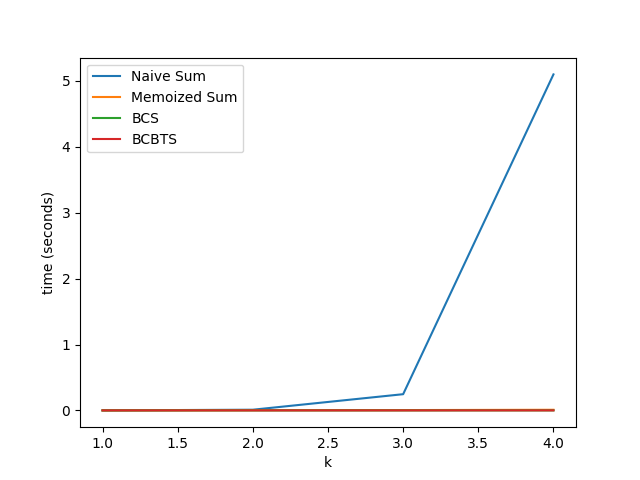
\includegraphics[scale=.7]{assets/1.png}    
\end{center}

\subsection{Excluding Memoized Sum}

Memoized Sum is very fast but it's intrinsically slower than BCS because BCS does not depend on $k$. Take a look at the same picture but for bigger $k$ and excluding the Naive Sum.

\begin{center}
    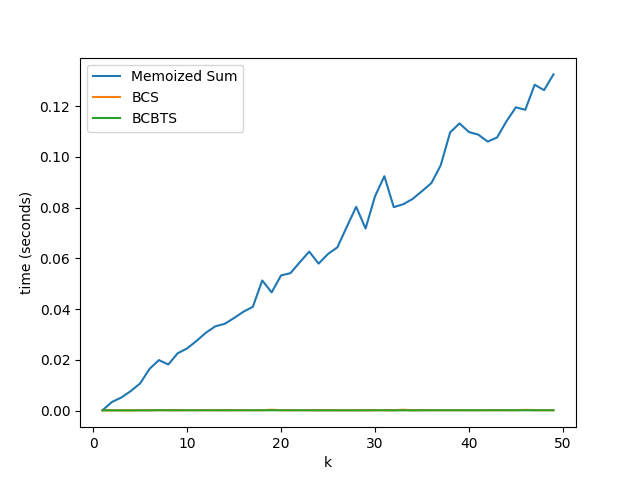
\includegraphics[scale=.8]{assets/2.png}
\end{center}

Note that Memoized Sum running time grows linearly with $k$ as expected.

\subsection{Big people fight: BCS vs BCBTS}

When talking about $k$, BCS takes the advantage because it does not depend on $k$. The following picture shows it.

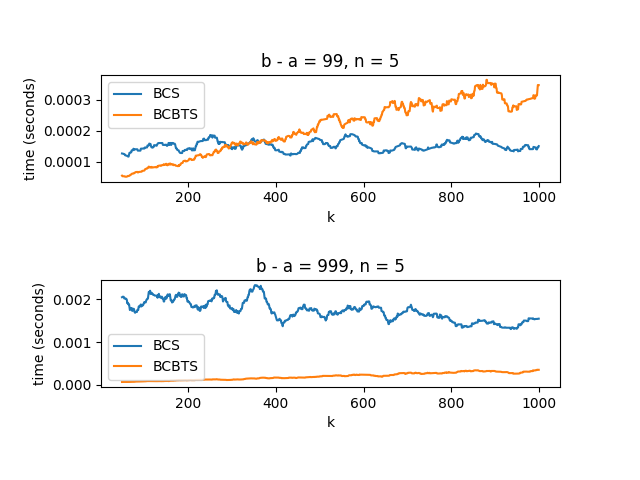
\includegraphics[scale=1]{assets/3.png}

However, BCBTS is faster when $b-a$ is big enough and $n$ small enough. That's why when talking about $b-a$, BCBTS is \textbf{absolutely} faster.

\begin{center}
    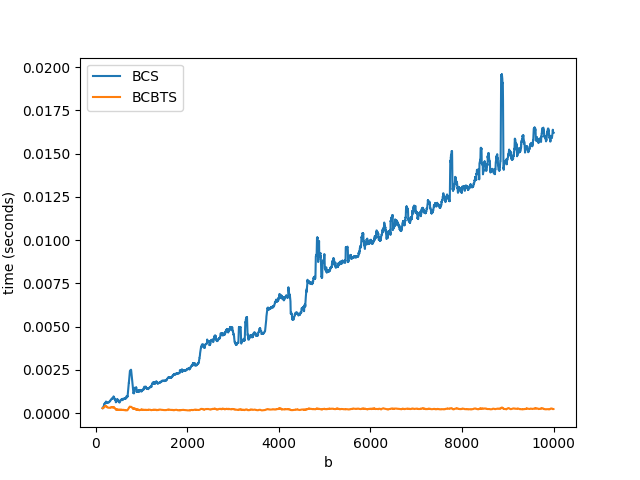
\includegraphics[scale=.7]{assets/4.png}
\end{center}

Note that BCS running time grows linearly with $b-a$, while BCBTS does not depend on $b-a$, as expected.

\section{Conclusion}

After demonstrations and speed comparisons, we conclude that BCS and BCBTS are super-fast algorithms that can improve significantly the calculation of nested sums of polynomials.

\vspace{10px}

BCS works for any function and does not depend on $k$. It's awesome! But if we are talking about polynomials, BCBTS is better for most cases. The only exception is if $b-a$ is small, $k$ is big and $n$ is big.

\end{document}